\documentclass{article}
% Comment the following line to NOT allow the usage of umlauts
\usepackage[utf8]{inputenc}
\usepackage[french]{babel}
\usepackage[a4paper, total={6in, 8in}]{geometry}
\usepackage{graphicx}
\usepackage{afterpage}
\usepackage{xcolor}
\usepackage[sfdefault,light]{roboto}
\usepackage[T1]{fontenc}
\usepackage{sectsty}
\usepackage[titles]{tocloft}
\usepackage{eso-pic}
\usepackage{fancyhdr}
\usepackage{pagecolor}

\definecolor{background}{HTML}{13181e}
\definecolor{green}{HTML}{32bba9}
\definecolor{greendark}{HTML}{16a085}


\sectionfont{\color{green}}  % sets colour of sections
\subsectionfont{\color{green}}  % sets colour of sections
\subsubsectionfont{\color{green}}
% \color{background}
% Start the document
\begin{document}

\makeatletter
    \begin{titlepage}
        \begin{center}
            \pagecolor{background}
            \color{white}
            
\includegraphics[width=0.5\linewidth]{assets/shape.png}\\[10ex]
            {\huge \bfseries BilleGateCoin - BGC}\\[2ex] 
            {\LARGE Scattered Corporation}\\[20ex]
            \large{by\\[2ex]aurele.oules  —  leo.gervoson  —  raphael.brenn  —  frederic.dong}\\[16ex] 
            {\large Projet EPITA 2020}
        \end{center}
    \end{titlepage}
\makeatother
\thispagestyle{empty}

\newpage
\begin{center}
\color{white}
\tableofcontents
\end{center}
\newpage
\pagecolor{white}
\sectionfont{\color{greendark}}  % sets colour of sections

\fancyhf{}
\renewcommand{\headrulewidth}{0pt}
\renewcommand{\footrulewidth}{1pt}
\newcommand\bold[1]{\textcolor{green}{\bfseries{#1}}}
\newcommand\boldblack[1]{\textcolor{background}{\bfseries{#1}}}
\renewcommand{\footrule}{\hbox to\headwidth{\color{green}\leaders\hrule height \footrulewidth\hfill}}

\lfoot{%
   \smash{%  % hide vertical stretch of the following content
    \parbox[b]{\textwidth}{%
    \raggedright
    \footnotesize
    
\includegraphics[width=0.08\linewidth]{assets/shape.png}\\[-7ex]
    }%
   }%
}
\rfoot{\thepage}
\pagestyle{fancy}
\renewcommand\seriesdefault{l}

% Create a new 1st level heading
\section{Introduction}
BilleGateCoin est une plateforme décentralisée pour un jeu de billes. Cette plateforme utilisera la technologie de la Blockchain pour sécuriser les parties. En 2008, Satoshi Nakamoto est le premier à résoudre le problème de la "double dépense" dans un système décentralisé : le Bitcoin. Cette technologie révolutionnaire et surprenante n'a cessé de prendre de plus en plus de place dans notre société. Nous avons décidé d'aborder cette technologie de la Blockchain de manière divertissante en l'appliquant à un jeu-vidéo dont les règles sont simples et les objets sont collectionnables : le jeu de billes.

\subsection{Membres}
\subsubsection{Aurèle}
Depuis que je suis tout petit, je suis passionné par la programmation et les jeux-vidéos. La Blockchain est une nouvelle technologie qui est encore en phase de développement et d'adoption. Ce projet de S2 à EPITA est l'occasion de montrer le potentiel de cette technologie émergente en l'appliquant au domaine du jeu vidéo. J'ai hâte de participer au développement de ce jeu original.

\subsubsection{Léo}
Ce projet m'intéresse d'une part car j'ai eu l'occasion d'en apprendre sur la blockchain lors des exposés d'anglais en présentant un exposé sur la blockchain, et d'autre part car je trouve l'utilisation de la blockchain pour la mise en place d'un jeu vraiment innovante et liant deux domaines habituellement séparés: les jeux et la blockchain.

\subsubsection{Raphaël}

Raphaël Brenn, 17 ans, j'ai une petite expérience en programmation (notamment pour des petits robots) et en modélisation 3D mais je n'avais jamais touché à Unity avant très récemment.

Je pense que créer ce type de jeu permet de montrer de façon concrète un autre secteur dans lequel il est possible d'utiliser la blockchain, par rapport à celui des crypto-monnaies, et plus largement expérimenter le développement d'un jeu vidéo selon un nouveau point de vue (ce qui permet à la fois de faire face à des problèmes inattendus, et contourner facilement d'autres problèmes qui auraient été plus gênants sans l'utilisation de cette technologie), ce que je trouve intéressant et 
potentiellement très enrichissant.

\subsubsection{Frédéric}

\subsection{Exemples}

Il existe plusieurs applications connues de la Blockchain :
\begin{itemize}
    \item Bitcoin : système bancaire décentralisé
    \item Ethereum : machine virtuelle pour éxécuter du code de manière décentralisée
    \item CryptoKitties : jeu décentralisé fonctionnant sur Ethereum dont le but est de collectionner des chats virtuels
\end{itemize}

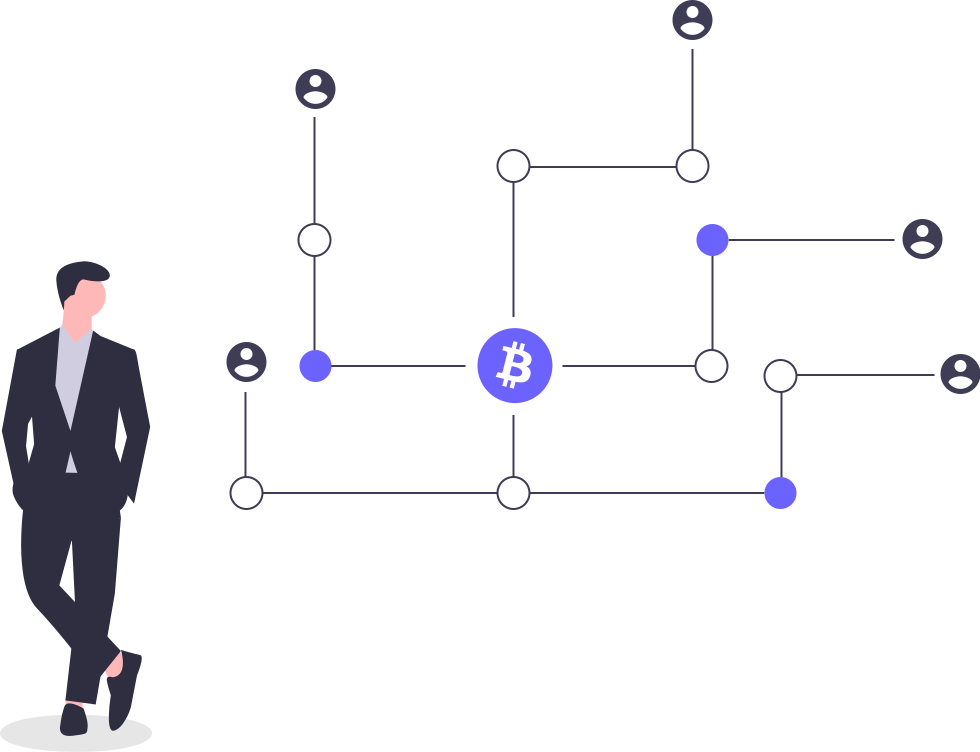
\includegraphics[width=0.3\linewidth]{assets/decentralized.png}\\

\subsection{Implémentation}

Le jeu de billes est un jeu classique dont le but est de collectionner des billes plus ou moins rares en combattant des adversaires ou en les échangeant. Une partie met en jeu les billes des joueurs : celui qui remporte la partie gagne la bille de son adversaire.

Chaque bille possède des propriétés physique différentes (adhérance, taille) et une rareté différente.
La façon la plus classique de jouer au jeu de billes est de lancer sa bille sur celle de l'adversaire pour gagner.


Dans l'implémentation de ce jeu, le joueur crée la partie avec un adversaire sélectionné.
Un terrain de jeu est généré avec des obstacles placés aléatoirement et les deux billes des joueurs sont placées de part et d'autre du terrain. Le joueur lance sa bille en direction de celle de l'adversaire. Si ce joueur touche sa bille, il la remporte. Sinon c'est au tour de l'adversaire de lancer sa bille. 

Nous allons évoquer les raisons de la décentralisation de la plateforme.

\section{Décentralisation}
La décentralisation de la plateforme offre une multitude d'avantages en comparaison à un système centralisé "normal".

\subsection{Confiance}
Les joueurs n'ont pas à faire confiance à une autorité centrale. 
\textit{Don't trust, verify.}

Le processus de création des billes ainsi que la définition de leur rareté est entièrement transparent et contrôlé par les joueurs mêmes, plutôt qu'une entreprise privée. Le taux de billes créées est fixé par les joueurs et personne ne peut le modifier sans le consensus général de la communauté. Personne ne peut confisquer les billes d'un joueur, même pas les développeurs.

\subsection{Point of Failure}
Dans un système décentralisé, il n'existe pas de point unique de défaillance (\textit{single point of failure}). 

Dans une plateforme centralisée, si le système est défaillant, tout le réseau est impacté. Contrairement à un système décentralisé où il ne suffit d'un seul ordinateur pour assurer la stabilité du réseau.

\subsection{Ouvert au développement}
N'importe quel individu avec des notions en programmation peut contribuer au développement de la plateforme.
Si assez de joueurs (consensus) acceptent ces changements alors ce code est ajouté à la plateforme.

Rien n'empêche un joueur de cloner cette plateforme afin de créer un jeu avec des règles différentes : \textit{Hard Fork}.

\section{Fonctionnement}
Afin de permettre la décentralisation du jeu, nous utiliserons la technologie de la Blockchain.

La \textit{Blockchain} est un régistre distribué (\textit{distributed ledger}) immuable et sécurisé par des milliers d'ordinateurs.

\subsection{Utilisateurs}
Sur une plateforme de jeu décentralisée, il n'y a pas de système de comptes avec une adresse email et un mot de passe.
Chaque joueur doit alors se générer une clé privée ainsi qu'une clé publique correspondante, avec un algorithme de cryptographie tels que RSA ou \textit{Elliptic Curve Digital Signature Algorithm} (ECDSA).

Cette clé privée doit être précieusement cachée car elle permet de signer toutes les transactions du joueur, c'est-à-dire créer une partie, lancer sa bille, échanger des billes, etc. L'utilisateur aura donc la possibilité de chiffrer sa clé privée sur son ordinateur et de la déchiffrer avec un mot de passe lors de la signature d'un contrat. 

\subsection{Lancement de la partie}
Deux modèles sont envisageables pour la création d'une partie.
\subsubsection{Deux étapes}
Le joueur choisit la bille qu'il veut jouer, son adversaire (sa clé publique) et la bille de son adversaire (qui lui appartient). Le joueur signe l'invitation avec sa clé privée et la diffuse sur la blockchain. L'adversaire reçoit alors une invitation pour créer cette partie, s'il accepte la partie, il doit également signer le contrat avec sa clé privée sur la blockchain. La partie commence.

Ce modèle assume que les deux joueurs n'ont pas de moyen de communication direct et utilisent la blockchain comme plateforme pour trouver des joueurs.

Ce modèle est couteux car il demande deux contrats sur la blockchain (création de la partie, et acceptation de la partie).


\subsubsection{Double signature}
Le joueur choisit la bille qu'il veut jouer, son adversaire (sa clé publique) et la bille de son adversaire (qui lui appartient). Le joueur signe ce contrat avec sa clé privée et demande à l'adversaire de signer également ce contrat avec sa clé privée. Une fois le contrat signé par les deux joueurs, le contrat est diffusé sur la blockchain. La partie commence.

Ce modèle assume que les deux joueurs ont un moyen de communication direct.

Ce modèle est moins couteux pour le joueur car l'accord entre les deux joueurs est fait hors-blockchain (\textit{off-chain}).
La création d'une plateforme centralisée permettant aux joueurs de trouver un accord est possible. La centralisation de cette plateforme ne pose pas de problèmes sur l'aspect décentralisé du jeu en lui-même.\\


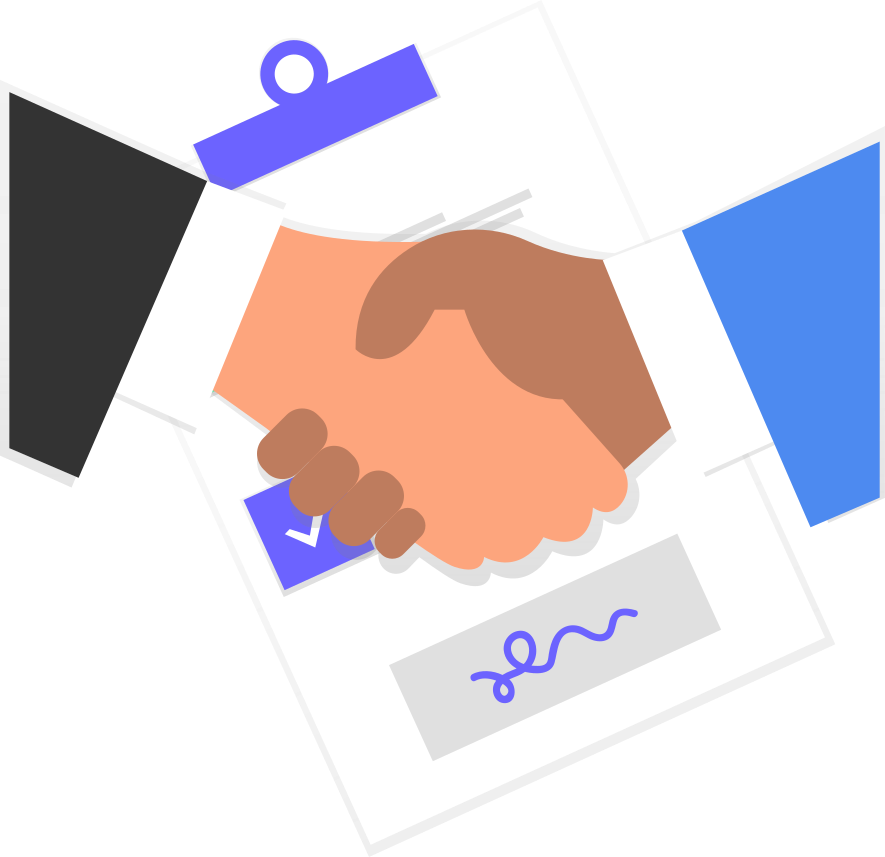
\includegraphics[width=0.3\linewidth]{assets/agreement.png}\\

Lors de la création de la partie, les joueurs doivent donner une ou plusieurs billes aux \textit{mineurs} afin de traiter la transaction (\textit{transaction fee}). Cette taxe permet aux mineurs d'être rémunérés pour leur travail. Nous implémenterons ce contrat à double signature plutôt que le précedent.


\subsection{Source d'entropie}
Lorsque la partie est créée, des obstacles sont aléatoirement placés sur le terrain pour ajouter de la difficulté au jeu de billes. Comme dans la vraie vie, il peut y avoir des trous, des arbres, des obstacles. Comment pouvons-nous générer un nombre aléatoire dans une Blockchain ?
Nous ne pouvons-pas générer de nombres aléatoires sur les nodes car le résultat serait différent pour tout le monde, alors nous devons utiliser une autre source d'entropie.

\subsubsection{Solution}

Lorsque le contrat de la création de la partie est signé, celui-ci est diffusé dans la \textit{mempool} des ordinateurs qui assurent la sécurité du réseau : \textit{nodes}. Les mineurs vont alors essayer de former un block avec les contrats et transactions de la mempool.

Pour se faire, les mineurs vont calculer un hash \textit{SHA-256} en concatenant toutes les valeurs du block telles que la date du block, les données de chaque contrat et l'indice du dernier block. Si ce block contient un certain nombre \textit{(mining difficulty)} de `0` en tête de hash, alors ce hash est valide et le block est dit "miné".

Ce hash n'est qu'un nombre hexadécimal aléatoire compris entre 1 et la \textit{mining difficulty}. Ce nombre va permettre la génération des obstacles la partie, en fonctionnant comme un \textit{seed}.

\subsubsection{Limites}
Toutes les parties créées dans ce block auront alors le même seed, c'est-à-dire l'exacte même répartition des obstacles.  

Il suffit de régler le \textit{block time} de la blockchain à un temps court pour permettre une génération de block plus rapide et donc des parties plus diversifiées. 

\subsection{Déroulement de la partie}
Une fois la partie créée, si le seed de la partie est pair c'est au joueur 1 de commencer, sinon c'est au tour du joueur 2.

Pour lancer sa bille, le joueur doit cliquer sur sa bille, et la tirer avec une certaine force. Un début de trajectoire s'affichera pour que le joueur puisse voir approximativement la direction de sa bille.
Une fois la bille lâchée, un vecteur force est créé. Le joueur doit alors signer ce vecteur force avec sa clé privée. Celui-ci est exécuté sur l'écran du joueur, il voit alors sa bille se déplacer. Le vecteur signé est également diffusé sur la Blockchain.

Les nodes et les mineurs vont vérifier la nouvelle position de la bille en fonction du vecteur signé par le joueur. Si la bille touche celle de l'adversaire alors la partie se termine et il remporte toutes les billes. Dans le cas contraire la partie continue et c'est au tour de l'autre joueur.

Pour éviter des problèmes de précision, la nouvelle position de la bille n'est jamais enregistrée dans la Blockchain. Ainsi pour déterminer l'état actuel de la partie (la position des deux billes) il faut recalculer la position de chaque bille grâce aux précédents vecteurs force signés par les joueurs respectifs.

Plus la partie est longue, plus le calcul de la position de la bille est coûteux en ressources, les taxes de transactions seront alors de plus en plus élevées. Les joueurs doivent se mettre d'accord en début de partie du nombre de tours maximum, si ce nombre est depassé pendant la partie, celle-ci se termine et les joueurs reprennent leur bille.

\subsection{Fin de partie}
Lorsqu'un joueur parvient à toucher la bille de l'autre, celui-ci gagne la partie. Pour récupérer ses gains (la bille de l'adversaire ainsi que sa propre bille), le joueur doit diffuser sur la blockchain une \textit{claim transaction}. Tant que le gagnant n'a pas diffusé cette transaction, il ne peut pas récupérer les mises.

Ainsi pour vérifier l'appartenance d'une bille, les nodes doivent uniquement parcourir la liste des \textit{claim transactions} au lieu de recalculer l'état de la partie et vérifier que les billes se touchent. 
Cela permet également de constituer rapidement l'historique d'appartenance de la bille. 

Ce contrat peut être diffusé uniquement si la partie est terminée, et la clé publique de la signature correspond à la clé publique du gagnant.

\subsection{Nodes}
Une \textit{node} est un ordinateur connecté à tout le réseau de la blockchain. Elle a un rôle majeur sur la sécurité du réseau.

\subsubsection{Arbitre}
La node possède le rôle d'arbitre.
Lorsque une partie est créée ou un joueur lance sa bille, la node va vérifier si le joueur possède bien cette bille, si c'est bien au tour du joueur de jouer, s'il n'essaye pas de lancer sa bille plus fort que la limite, etc.
Si le contrat est valide, celui-ci rentre dans la \textit{memory pool} de la node, sinon il est rejeté.

\subsubsection{Régistre}
La node s'occupe de stocker l'historique entier de toutes les parties et transactions de tous les joueurs, c'est-à-dire la blockchain.

L'ordinateur réserve également un emplacement pour stocker les transactions non confirmées par les mineurs, c'est-à-dire les lancés de billes et créations de parties qui viennent d'être diffusées par les joueurs. Cet emplacement s'appelle la \textit{memory pool}.

\subsubsection{Distribution}
Le rôle principal de la node est de partager la blockchain à toutes les autres nodes du réseau. 
La node qui possède la plus grande chaîne est celle qui possède la chaîne la plus valide, elle doit donc la partager au réseau.

\subsection{Mineurs}
Les mineurs assurent l'immuabilité de la blockchain.
Un block contient des contrats et des lancés de billes. Pour ajouter un block à la blockchain, un puzzle constitué exclusivement des données du block doit être résolu. Ce puzzle n'est solvable uniquement en essayant des milliards de combinaisons par secondes.

\subsubsection{Block hash}

Un hash\footnote{Une fonction hash est une fonction qui prend une entrée telle que du texte ou un nombre, et retourne un nombre qui apparaît aléatoire mais est déterministe. Pour la même entrée, la fonction retournera toujours la même sortie. C'est une fonction à sens unique, le hash ne permet pas de retrouver l'entrée.} SHA-256 est un nombre hexadécimal aléatoire compris entre 1 et $2^{256} - 1$.

La solution du puzzle que les mineurs doivent résoudre est en réalité un hash du block qui doit être compris entre 1 et $\frac{2^{256}-1}{mining\ difficulty}$.

Les mineurs forment un block à partir des contrats de la \textit{memory pool} des nodes.

Si le hash n'est pas compris dans cet intervalle, les mineurs calculent à nouveau un hash du block en concatenant un \textit{nonce} différent. C'est un nombre arbitraire qui permet uniquement de générer un hash différent en conservant les valeurs du block.

Ce hash sécurise la blockchain car il est facile de le résoudre si tout le réseau travail sur ce problème, mais il est impossible de résoudre ce problème seul. Ce système assume que plus de 50\% du réseau est honnête.

Si un utilisateur malveillant voulait essayer de falsifier une transaction en l'ajoutant soi-même à la blockchain, c'est-à-dire en minant le block soi-même, il devrait alors résoudre ce puzzle extrêmement compliqué seul. De plus, aucune node n'accepterai cette transaction, sauf si l'utilisateur possède plus de la moitié des ordinateurs du réseau (\textit{51\% attack}) car l'utilisateur pourrait ainsi corrompre le consensus et former une nouvelle blockchain.
Cette attaque est extrêmement peu probable.

\subsubsection{Ajustement de la difficulté}

La difficulté de minage est une variable qui assure que les mineurs ajoutent des blocks à la blockchain de manière régulière même si le nombre de mineurs, donc de puissance de calcul, augmente.
 
Cette difficulté permet aux nodes de prévoir l’espace disque nécessaire pour stocker la blockchain et assure une économie stable (voir section suivante). Elle doit donc être ajustée régulièrement.

Le \textit{block time} est une constante qui définit le temps qu’un mineur met pour ajouter un block à la chaîne.

Sur la plateforme de jeu de billes, le block time doit être assez court (entre 20s et une minute) afin de permettre des exécutions de contrats (créations de parties, et lancés de billes) rapides. Par exemple, le Bitcoin utilise un block time de 10 minutes, et Ethereum un block time de 20 secondes.

Un intervalle trop court peut causer des problèmes sur le délai de distribution des nouveaux blocks entre les nodes.

La difficulté de minage est au départ 1. Celle-ci est ajustée tous les X
blocks. Chaque node va calculer le temps que X block prennent pour être minés en théorie, divisé par la moyenne de temps que les X derniers blocks ont pris pour être minés. La difficulté est ainsi multipliée par ce coefficient.

\[ nouvelle\ difficult\acute{e} = difficult\acute{e} \times \frac{temps\ attendu}{temps\ r\acute{e}el} \]

\subsubsection{Récompenses}
Dans chaque block miné, le mineur inclut une transaction spéciale : la \textit{coinbase transaction}. C'est la récompense du mineur.
Cette transaction n'a pas d'input, uniquement l'adresse publique du mineur pour recevoir sa récompense.
Celle-ci contient de nouvelles billes créées, toutes plus ou moins rares telles que 1000 billes grises, 100 billes bleues, et 50 billes rouges. Les rouges seraient par définition plus rares que les autres car il y en aurait moins en circulation.
En plus de ces nouvelles billes, le mineur récupère toutes les taxes des transactions de chaque joueur (sous la forme de billes également).

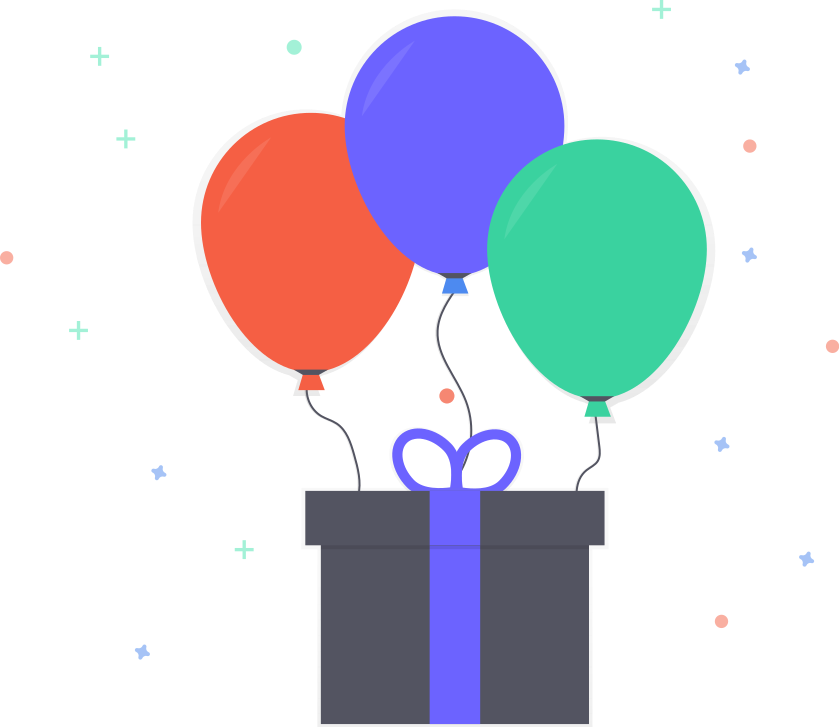
\includegraphics[width=0.3\linewidth]{assets/gift.png}\\

Tous les X blocks (210 000 blocks pour Bitcoin $\approx$ 4\ ans), les récompenses des mineurs sont divisées par deux jusqu'à que la totalité des billes soient distribuées.
La prochaine récompense serait de 500 billes grises, 50 billes bleues, et 25 billes rouges.

\section{Contrats}
\subsection*{Placement de billes}
\hspace*{-1cm}%
\begin{tabular}{ |c|c|c|c|c|c|c|c|c| } 
 \hline
octets & 1 & 1 & 8 & ... & 1 & 8\\ 
 \hline
    données & \# types & type & quantité & ... & type & quantité \\ 
 \hline
\end{tabular}
\subsection{Création de la partie}
\subsubsection{Double signature}
\hspace*{-1cm}%
\begin{tabular}{ |c|c|c|c|c|c|c|c|} 
 \hline
 octets & 1 & 1 & ? & ? & ? & 8 & 128\\ 
 \hline
    données & version & type contrat & taxe (billes) & billes J1 & billes J2 & nonce & signatures\\ 
 \hline
\end{tabular}

\subsubsection{Invitation et acceptation}
\hspace*{-1cm}%
\begin{tabular}{ |c|c|c|c|c|c|c|c|c|} 
 \hline
 octets & 1 & 1 & ? & 20 & ? & ? & 8 & 64\\ 
 \hline
    données & version & type contrat & taxe (billes) & adresse J2 & billes J1 & billes J2 & nonce & signature\\ 
 \hline
\end{tabular}\\ \break

\hspace*{-1cm}%
\begin{tabular}{ |c|c|c|c|c|c|c|} 
 \hline
 octets & 1 & 1 & ? & 32 & 8 & 64\\ 
 \hline
    données & version & type contrat & taxe (billes) & contrat ID & nonce & signature\\ 
 \hline
\end{tabular}

\subsection{Lancé de bille}
\hspace*{-1cm}%
\begin{tabular}{ |c|c|c|c|c|c|c|c|c|} 
 \hline
 octets & 1 & 1 & ? & 1 & 1 & 32 & 8 & 64 \\ 
 \hline
    données & version & type contrat & taxe (billes) & second & Z & contrat ID & nonce & signature\\ 
 \hline
\end{tabular}

\subsection{Claim transaction}
\hspace*{-1cm}%
\begin{tabular}{ |c|c|c|c|c|c|c|c|} 
 \hline
 octets & 1 & 1 & ? & 32 & 20 & 8 & 64 \\ 
 \hline
    données & version & type contrat & taxe (billes) & contrat ID & adresse & nonce & signature\\ 
 \hline
\end{tabular}

\subsection{Échange (double signature)}
\hspace*{-1cm}%
\begin{tabular}{ |c|c|c|c|c|c|c|c|} 
 \hline
 octets & 1 & 1 & ? & ? & ? & 8 & 128\\ 
 \hline
    données & version & type contrat & taxe (billes) & billes J1 & billes J2 & nonce & signatures\\ 
 \hline
\end{tabular}

\section{Jeu}
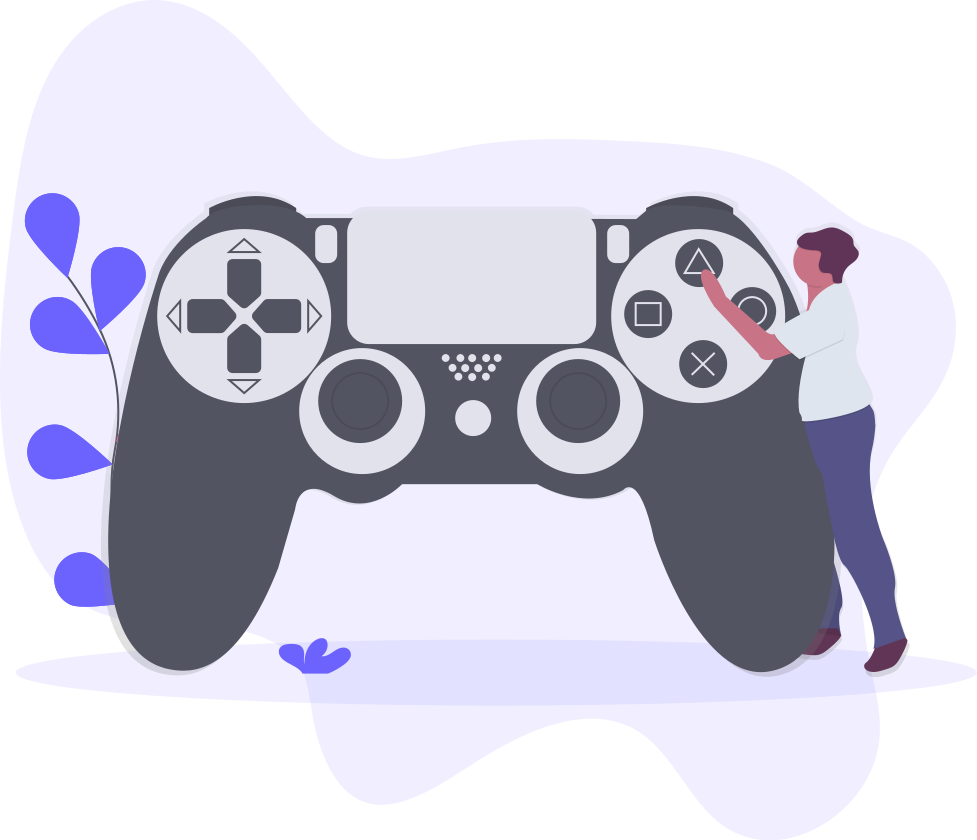
\includegraphics[width=0.3\linewidth]{assets/gaming.png}\\
\subsection{Menus}

Lors du lancement du jeu, un menu principal apparait. Des boutons apparaissent:
\begin{itemize}
    \item Parties en cours
    \item Nouvelle partie
    \item Collection
\end{itemize}

\subsubsection{Parties en cours}
Une nouvelle page s'affiche avec les parties en cours de l'utilisateur (sa clé publique). Le joueur peut voir le nombre de coups déjà joués, les billes mises en jeu, la clé publique de son adversaire et l'état actuel de la partie.

Si c'est au joueur de jouer, il peut alors cliquer sur un bouton pour continuer la partie. Le terrain de la partie se génère et il peut lancer sa bille.

\subsubsection{Nouvelle partie}
Lorsque le joueur clique sur le bouton Nouvelle partie, une nouvelle page s'ouvre avec:
\begin{itemize}
    \item La clé publique de l'adversaire
    \item Une boîte de séléction de la/les billes qu'il veut jouer
    \item Une boîte de sélection de la/les billes de l'adversaire
    \item Une boîte de sélection de la/les billes qu'il donne aux mineurs (transaction fee)
\end{itemize}

Le joueur devra signer ce contrat avec sa clé privée avec une boîte de dialogue lui demandant son mot de passe. Celui-ci devra faire signer ce contrat à l'adversaire. Une fois le contrat signé par les deux parties, ce contrat peut être diffusé sur la blockchain par un des deux joueurs. La partie commence.

\subsubsection{Collection}
Le joueur pourra voir sa collection de billes en cliquant sur le bouton Collection sur le menu d'accueil. Il pourra également examiner les propriétés physique de chaque billes et leur rareté.

\subsection{Gameplay}
Les terrains du jeu sont générés en fonction d'un \textit{seed}. Pour le même seed, la répartition des billes et des obstacles seront sera toujours la même le même.

Une physique déterministe sera implémentée. Pour un lancé de bille quelconque, la nouvelle position de la bille doit toujours être la même peu importe la marque du processeur de l'utilisateur, sa rapidité, l'heure, etc. Cela permet aux \textit{nodes} d'obtenir le même résultat peu importe le contexte, et donc d'arbitrer la partie avec une haute précision.


\section{Outils et coûts}
Nous allons utiliser de nombreux outils durant le développement de ce projet.

\subsection{Développement global}
Les principaux outils que nous utiliserons seront :

\begin{itemize}
    \item C\#
    \item Git
    \item GitHub
    \item Travis-CI
    \item \LaTeX
    \item Discord
    \item Google

\end{itemize}

\subsection{Développement de la blockchain}
Nous utiliserons différents éditeurs de code tels que VIM, VS Code, ou Rider.

Nous utiliserons les technologies suivantes pour le développement de la blockchain :
\begin{itemize}
\begin{samepage}
    \item LevelDB : base de données clé/valeur
    \item ECDSA : algorithme de signature digitale
    \item SHA-256 : algorithme de hash
\end{samepage}
\end{itemize}

\subsection{Développement du jeu}

Les logiciels suivants nous aideront durant le développement du jeu :
\begin{itemize}
    \item Unity
    \item Adobe Photoshop
    \item Blender
\end{itemize}

\subsection{Developpement du site web}
Les technologies suivantes nous aideront durant le développement du site web :
\begin{itemize}
    \item Netlify
    \item React.js
    \item Sass
    \item MongoDB / MySQL
    \item Google Chrome
\end{itemize}

\subsection{Coûts}
\begin{center}
\setlength{\tabcolsep}{15pt}
\renewcommand{\arraystretch}{1.8}

\hspace*{-1cm}%
\begin{tabular}{ |c|c|c|c|} 
 \hline
    \boldblack{Élément} & \boldblack{Prix} & \boldblack{Quantité} & \boldblack{Description}\\ 
     \hline
        Hébergement des serveurs & 0.00€ & $\infty$ & C'est pas décentralisé pour rien \\ 
     \hline
        Nom de domaine & 0.00€ & 1 & Offert par GitHub Student Pack \\ 
     \hline
        Discord & 0.00€ & - & - \\ 
     \hline
        GitHub & 0.00€ & - & - \\ 
     \hline
        Électricité & 0.1452€ & / kWh & - \\ 
     \hline
     \end{tabular}
\end{center}

\setlength{\tabcolsep}{15pt}
\renewcommand{\arraystretch}{1.8}

\section{Tâches}
\subsection{Répartition des tâches}
\begin{center}
\hspace*{-1cm}%
\begin{tabular}{ |c|c|c|c|c|} 
 \hline
    \boldblack{tâche} & \boldblack{Aurèle} & \boldblack{Léo} & \boldblack{Raphaël} & \boldblack{Frédéric} \\ 
     \hline
    Génération clées privées (ECDSA) & second & \bold{principal} &  & \\ 
     \hline
     Création de porte-feuille & \bold{principal} & second &  & \\ 
     \hline
    Mining (Proof of Work) & \bold{principal} & second &  & \\ 
     \hline
     Merkle Tree & \bold{principal} & second &  & \\ 
     \hline
    Récompenses des mineurs & second & \bold{principal} & & \\ 
     \hline
    Encodage/décodage contrats & \bold{principal} & second &  & \\ 
     \hline
    Signature contrats & second & \bold{principal} &  & \\ 
     \hline
    Command Line Interface (CLI) & second & \bold{principal} & &\\ 
     \hline
    Module de persistance (LevelDB) & \bold{principal} & second &  & \\ 
     \hline
     Communication tcp/ip & second & \bold{principal} &  & \\ 
     \hline
    Memory Pool & second & \bold{principal} &  & \\ 
     \hline
     Application des règles du jeu (consensus) & \bold{principal} & second &  & \\ 
     \hline
     Définition des 256 billes (nom, atoûts, rareté) & & & second & \bold{principal}\\ 
    \hline
    Design des billes & second & & \bold{principal} & \\ 
     \hline
    Menus du jeu & & & second & \bold{principal}\\ 
     \hline
    Interface de selection de billes & & & second & \bold{principal}\\ 
     \hline
     Modélisation 3D des obstacles & & & \bold{principal} & second\\ 
     \hline
     Création du plateau de jeu (avec seed) & & second &  & \bold{principal}\\ 
     \hline
      Lancement de la bille & & & \bold{principal} & second\\ 
    \hline
       Physique deterministe (Unity DPhysics) & & & second & \bold{principal} \\ 
     \hline
    Détection collision de victoire & & & \bold{principal} & second\\ 
     \hline
    Site web & \bold{principal} & & & second\\ 
     \hline
\end{tabular}
\end{center}

\setlength{\tabcolsep}{9pt}
\renewcommand{\arraystretch}{2}

\subsection{Objectifs}
\begin{center}
\hspace*{-1cm}%
\begin{tabular}{ |c|c|c|c|} 
 \hline
    \boldblack{tâche} & \boldblack{1ère soutenance} & \boldblack{2ème soutenance} & \boldblack{3ème soutenance}\\ 
     \hline
        Génération d'un porte-feuille fonctionnel & \bold{100\%} & / & / \\ 
     \hline
        Encodage / Décodage des contrats & \bold{100\%} & / & / \\ 
     \hline
        Signature contrats & \bold{100\%} & / & / \\ 
    \hline
        Mining & 33\% & 66\% & \bold{100\%} \\ 
     \hline
        Memory Pool & 50\% & \bold{100\%} & / \\ 
     \hline
        Récompenses & 0\% & 50\% & \bold{100\%} \\ 
     \hline
        CLI & 33\% & 66\% & \bold{100\%} \\ 
     \hline
        Module de persistance & 50\% & \bold{100\%} & / \\ 
     \hline
        Communication TCP/IP & 0\% & 50\% & \bold{100\%} \\ 
     \hline
        Définition des billes & 33\% & 66\% & \bold{100\%} \\ 
     \hline
        Design des billes & 33\% & 66\% & \bold{100\%} \\ 
     \hline
        Menus du jeu & 50\% & \bold{100\%} & / \\ 
     \hline
        Modélisation 3D & 0\% & 50\% & \bold{100\%} \\ 
     \hline
        Terrain de jeu & 33\% & 66\% &\bold{100\%} \\ 
     \hline
         Lancés et trajectoires & 33\% & 66\% &\bold{100\%} \\ 
     \hline
         Site web & 0\% & 50\% &\bold{100\%} \\ 
     \hline
     \end{tabular}
\end{center}

\section{Conclusion}
BilleGateCoin est un projet ambitieux et un défi pour tous les membres de \bold{Scattered Corp}. Malgré l'aspect simple du jeu de billes, le but de ce projet est de créer un jeu vidéo entièrement transparent afin de complètement réduire le niveau de confiance que les joueurs doivent donner aux développeurs de la plupart des jeux vidéos d'aujourd'hui.


\end{document}
